\section{Date: 2026-10-15}
\noindent \textbf{Series ID: PLGCPPSEA670NRUG} 

\noindent This series is titled Price Level of Government Consumption for Sweden and has a frequency of Annual. The units are Price Level of USA Output-side GDP in 2021=1 and the seasonal adjustment is Not Seasonally Adjusted.The observation start date is 1950-01-01 and the observation end date is 2023-01-01.The popularity of this series is 1. \\ 

\noindent \textbf{Series ID: CUUSA214SEHF} 

\noindent This series is titled Consumer Price Index for All Urban Consumers: Energy Services in Kansas City, MO-KS (CMSA) (DISCONTINUED) and has a frequency of Semiannual. The units are Index 1982-1984=100 and the seasonal adjustment is Not Seasonally Adjusted.The observation start date is 1984-01-01 and the observation end date is 2017-07-01.The popularity of this series is 1. \\ 

\subsection{Raw Regression}
\noindent Regresses the two series against each other directly. A significant result here can come just as easily from both series sharing a long-run trend as from any real relationship.

\begin{center}
\begin{tabular}{lclc}
\toprule
\textbf{Dep. Variable:}                & value\_fred\_CUUSA214SEHF & \textbf{  R-squared:         } &     0.326   \\
\textbf{Model:}                        &            OLS            & \textbf{  Adj. R-squared:    } &     0.305   \\
\textbf{Method:}                       &       Least Squares       & \textbf{  F-statistic:       } &     15.50   \\
\textbf{Date:}                         &      Thu, 15 Oct 2026     & \textbf{  Prob (F-statistic):} &  0.000418   \\
\textbf{Time:}                         &          15:51:08         & \textbf{  Log-Likelihood:    } &   -162.19   \\
\textbf{No. Observations:}             &               34          & \textbf{  AIC:               } &     328.4   \\
\textbf{Df Residuals:}                 &               32          & \textbf{  BIC:               } &     331.4   \\
\textbf{Df Model:}                     &                1          & \textbf{                     } &             \\
\textbf{Covariance Type:}              &         nonrobust         & \textbf{                     } &             \\
\bottomrule
\end{tabular}
\begin{tabular}{lcccccc}
                                       & \textbf{coef} & \textbf{std err} & \textbf{t} & \textbf{P$> |$t$|$} & \textbf{[0.025} & \textbf{0.975]}  \\
\midrule
\textbf{const}                         &      51.5366  &       22.372     &     2.304  &         0.028        &        5.966    &       97.107     \\
\textbf{value\_fred\_PLGCPPSEA670NRUG} &      84.4492  &       21.453     &     3.937  &         0.000        &       40.752    &      128.147     \\
\bottomrule
\end{tabular}
\begin{tabular}{lclc}
\textbf{Omnibus:}       &  0.731 & \textbf{  Durbin-Watson:     } &    0.224  \\
\textbf{Prob(Omnibus):} &  0.694 & \textbf{  Jarque-Bera (JB):  } &    0.812  \\
\textbf{Skew:}          &  0.276 & \textbf{  Prob(JB):          } &    0.666  \\
\textbf{Kurtosis:}      &  2.482 & \textbf{  Cond. No.          } &     8.76  \\
\bottomrule
\end{tabular}
%\caption{OLS Regression Results}
\end{center}

Notes: \newline
 [1] Standard Errors assume that the covariance matrix of the errors is correctly specified.

\begin{figure}
\centering
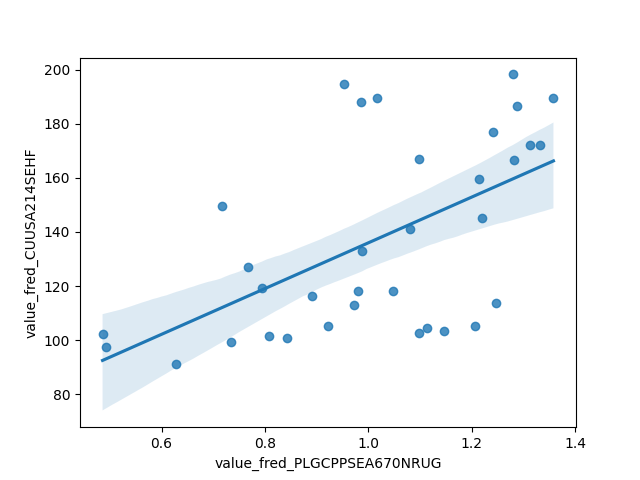
\includegraphics[scale = 0.9]{plots/plot_2026-10-15.png}
\caption{Raw Regression Plot for 2026-10-15}
\end{figure}
\newpage
\subsection{Detrended Regression}
\noindent Regresses the residuals of each series after removing its own linear time trend, so a shared trend can no longer drive the result on its own. A relationship that stays significant here is better evidence of a genuine link between the two series.

\begin{center}
\begin{tabular}{lclc}
\toprule
\textbf{Dep. Variable:}                           & value\_fred\_CUUSA214SEHF\_detrended & \textbf{  R-squared:         } &     0.006   \\
\textbf{Model:}                                   &                 OLS                  & \textbf{  Adj. R-squared:    } &    -0.025   \\
\textbf{Method:}                                  &            Least Squares             & \textbf{  F-statistic:       } &    0.1907   \\
\textbf{Date:}                                    &           Thu, 15 Oct 2026           & \textbf{  Prob (F-statistic):} &    0.665    \\
\textbf{Time:}                                    &               15:51:08               & \textbf{  Log-Likelihood:    } &   -126.43   \\
\textbf{No. Observations:}                        &                    34                & \textbf{  AIC:               } &     256.9   \\
\textbf{Df Residuals:}                            &                    32                & \textbf{  BIC:               } &     259.9   \\
\textbf{Df Model:}                                &                     1                & \textbf{                     } &             \\
\textbf{Covariance Type:}                         &              nonrobust               & \textbf{                     } &             \\
\bottomrule
\end{tabular}
\begin{tabular}{lcccccc}
                                                  & \textbf{coef} & \textbf{std err} & \textbf{t} & \textbf{P$> |$t$|$} & \textbf{[0.025} & \textbf{0.975]}  \\
\midrule
\textbf{const}                                    &    1.842e-12  &        1.763     &  1.05e-12  &         1.000        &       -3.590    &        3.590     \\
\textbf{value\_fred\_PLGCPPSEA670NRUG\_detrended} &      -4.1498  &        9.502     &    -0.437  &         0.665        &      -23.505    &       15.205     \\
\bottomrule
\end{tabular}
\begin{tabular}{lclc}
\textbf{Omnibus:}       &  0.585 & \textbf{  Durbin-Watson:     } &    1.001  \\
\textbf{Prob(Omnibus):} &  0.746 & \textbf{  Jarque-Bera (JB):  } &    0.498  \\
\textbf{Skew:}          &  0.275 & \textbf{  Prob(JB):          } &    0.780  \\
\textbf{Kurtosis:}      &  2.781 & \textbf{  Cond. No.          } &     5.39  \\
\bottomrule
\end{tabular}
%\caption{OLS Regression Results}
\end{center}

Notes: \newline
 [1] Standard Errors assume that the covariance matrix of the errors is correctly specified.

\begin{figure}
\centering
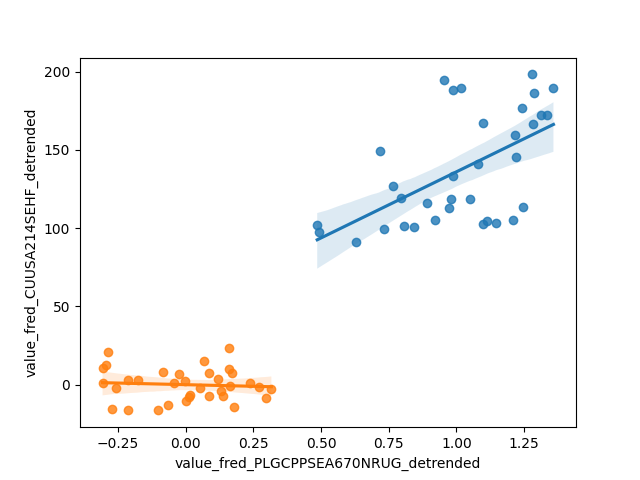
\includegraphics[scale = 0.9]{plots/plot_2026-10-15_detrended.png}
\caption{Detrended Regression Plot for 2026-10-15}
\end{figure}
\newpage
